\chapter{Introduction}\label{ch:introduction}


\section{Artificial intelligence}

\newglossaryentry{ai}{name={AI},description={Artificial intelligence}}

The development of the early $21^{\text{st}}$ century was largely shaped by the transformative influence of information technology, and on its frontier is  Artificial intelligence (\gls{ai}).
Ever since the development of the Google search engine at the beginning of the century, numerous \gls{ai} algorithms have been used to aid tasks typically done by humans.
Its influence is particularly evident in the changing landscape of today's economy.
Forbes' Fortune 500 list, ranking the most successful companies worldwide, was typically dominated by oil companies in the $20^{\text{th}}$ century.
In recent years, the dominion has shifted towards the IT companies; among the ten most valuable companies, five are IT -- Apple, Alphabet, Microsoft, Amazon and Facebook.
Although we can say that the \gls{ai} is the core business only for the Alphabet's subsidiary Google, \gls{ai} is present in the ever increasing number of products of the other companies.







% TODO: add references to claims
Despite its importance, it is still difficult to say what \gls{ai} precisely is.
One of the most common definitions describes \gls{ai} as building \textit{machines that think like humans}.
However, this definition is not operative as we still do not understand how the humans think.
A more operative definition is that of \gls{ai} creating \textit{machines that behave intelligently}.
This  way \gls{ai} machines only have to act intelligently and does not require understanding the human intelligence nor the peculiarities of various problem solving skills humans posses.
Like human intelligence, \gls{ai} is a broad field including many different tasks.
Examples include problems of planning and scheduling, automated reasoning, theorem proving, robotics, language understanding and many others.
Many problems within AI often require a combination of different methods.
The latest two decades have also witnessed many breakthrough application of AI including DeepBlue \cite{Hsu:2002:BDB:601291}  which defeated the world chess champion Gary Kasparov, Watson \cite{journals/aim/FerrucciBCFGKLMNPSW10} which has defeated the top human players in the question-answering game of Jeopardy!, AlphaGo \cite{SilverHuangEtAl16nature,silver2017mastering} which has dominated the best human player in the game of Go, self-driving cars and many more.





\section{Machine learning and logic}
\label{sec:intro_ml}

\newglossaryentry{ml}{name={ML},description={Machine Learning}}
\newglossaryentry{srl}{name={SRL},description={Statistical relational learning}}
\newglossaryentry{ilp}{name={ILP},description={Inductive logic programming}}

One aspect that made \gls{ai} influential is the growing number of digital devices and the amount of information they produce and store.
Extracting useful information from the massive available data has the potential to reveal patterns and insights about many aspects of the everyday life.
This is, in a way, similar to the tests designed by psychologists and sociologists interrogating the nature of individuals and society, with a difference that the starting point is not a design of a questionnaire but the available data.
This way \gls{ai} has changed our perspective in data, which has been transformed from a mere record of an event to a carrier of useful information.

Perhaps the most prominent representative of \gls{ai} nowadays is machine learning (\gls{ml}), which concerns extraction of useful patterns from data.
Machine learning develops \gls{ai} systems that \textit{improve their performance with experience}.
This means that systems learn concepts and skills from examples -- the data provided by the expert, or through interaction with the environment.
These systems are therefore not programmed in advance; rather, their skills are acquired from the examples.
The impact of such systems is huge: from discovering new knowledge to bringing the power of computer programming to non-experts which could simply show the computer how to solve the task, instead of programming it.



How exploiting such data has influenced the modern world is perhaps best summarised  in a quote by the mathematician Clive Humbly:
\begin{quote}
	Data is the new oil. It’s valuable, but if unrefined it cannot really be used. It has to be changed into gas, plastic, chemicals, etc to create a valuable entity that drives profitable activity; so must data be broken down, analysed for it to have value.
\end{quote}




A common idea underlying many machine learning algorithms is that of learning a \textit{model of the world}.
This assumes that a learning task is defined as a system with clearly defined inputs and outputs.
Given these inputs and outputs, a task of a typical machine learning algorithm is to discover a \textit{decision function}, a system's gearwheels transforming the inputs to the output(s).
Existing machine learning algorithms differ in the gearwheels they use to solve the task, i. e., how they \textit{represent} a decision function.






\begin{table}
	\centering
	\caption[An example dataset]{An example dataset describing pets, their features (columns one to six) and the target concept}
	\resizebox{0.95\textwidth}{!}{
		\begin{tabular}{@{}lccccccc@{}}
			\toprule
			\textbf{ID} &\multicolumn{6}{c}{\textbf{Features}} 									& \textbf{Target} \\
			\cmidrule(lr){2-7}
						& legs	& fluffiness		& diary 		& playful	& spits? 	& bites? 	&	\\
			\midrule
			cat			& 4		& 4				& carnivore	& sometimes & no		 	& sometimes	&  \checkmark \\
			dog			& 4		& 5				& carnivore	& yes		& no		& no		& \checkmark \\
			duck		& 2		& 2				& herbivore	& no			& no		& no		& $\times$ \\
			\multicolumn{8}{c}{\ldots} \\
			alpaca		& 4		& 5				& herbivore & yes		& sometimes	& no		& ? \\
			\bottomrule
		\end{tabular}
	}
	\label{tab:pets}
\end{table}



\paragraph{Example (The art of machine learning in a nutshell)} Imagine yourself choosing a new pet.
Being an \gls{ai} enthusiast, and having to choose among a vast variety of potential pets, you decide to use a machine learning algorithm to help you with the decision.
The first challenge you are faced with  is getting the data.
You decide to compile a large database of potential pets and identify their \textit{features} -- for example, the number of legs, level of fluffiness of their fur, their diary, whether they are playful of not, and whether they spit or bite.
These features define the \textit{inputs} for a machine learning algorithm.
We still have to provide the \textit{experience} to the learning algorithm in form of the desired outputs; the input data (the features) and the desired output which define the learning task.
The desired output come from the previous pets you owned and whether you liked having them as pets or not -- for example, imagine you have own a dog and a cat which you liked, and a duck which you were not so fond of.
These examples constitute our \textit{training data}, and are compiler in a simple Excel sheet (Table \ref{tab:pets}).



Once the data is compiled, you can proceed with learning the  mapping the inputs to the outputs -- the decision function.
This faces you with the second choice -- how should the decision function look like?
The straightforward choice seems to be a form of \texttt{IF-THEN} rules:
\begin{center}
	\texttt{IF} legs $=$ 4 \texttt{AND} fluffiness $\geq 4$ \texttt{THEN} yes.
\end{center}
An alternative option would be to assign an \textit{importance} to each feature so that a desirable potential pet gets a positive score, while the un-desirable one gets a negative score:

$$ w_1 \cdot \text{legs} + w_2 \cdot \text{fluffiness} + w_3 \cdot \text{diary} + w_4 \cdot \text{playful} - w_5 \cdot \text{spits} - w_6 \cdot \text{bites} - w_7 \geq 0$$

In this case, we would have to replace categorical choices, such as \texttt{playful} feature, with a numerical equivalent.
For example, we could replace \texttt{no} with 0, \texttt{sometimes} with 1 and \texttt{yes} with 2.
Many choices are possible, and the right one depends on the task at hand.


Once the model has been learned, either by finding the rules or by tuning the weights of the decision function, the model can be applied to make decision about new examples.
For instance, if we wish to know whether an alpaca would make a good pet, we can ask the model.
Looking at the first rule, the answer would be \texttt{yes} as alpaca has four legs and the level of fluffiness above 4.



As the example demonstrates, it is necessary to differentiate between the representation of \textit{data} and the representation of  the \textit{decision function}.
This thesis focuses on the data representation aspect and inherits the representation of decision functions from the existing methods.





The choice of data representation involves two issues.
First, one has to decide about the data representation \textit{format}.
Data format describe the basic form -- a template, the data will take.
By far the most popular choice is the \textit{tabular representation}, e.g., Excel sheets, but other options include graphs, networks and even programming languages.
The second issue is concerned with the \textit{content} of the data itself, i.e., defining the \textit{features} of the task.
This populates the template with the content.



Both data representation aspects have a critical impact on the success of the machine learning application.
Choosing an insufficient data format prevents us from capturing all intricacies of the data.
Even more crucial is the choice of the features.
If the features themselves do not contain the information, no \gls{ml} algorithm will be able to successfully solve the task.
In contrast, insufficient data format might not be able to capture \textit{everything} about the data, but it is possible that it capture \textit{most} of the relevant information.



Identifying the right and informative features for the given problem is no easy task.
Developing a \gls{ml} model typically proceeds in four steps: 1) collecting the data, 2) designing the features, 3) learning the model, and 4) evaluating the model.
However, this is rarely a linear procedure; the practitioners typically have to iterate between steps 2 and 4 to find the suitable features, resulting in a labour-intensive task taking the vast majority of the development [citation?].
The main reason why finding the informative features is difficult is that one typically uses machine learning algorithm to solve the task the one does not know how to solve.
As the solution is unknown, it is even more difficult to know which information has to be a part of the solution.


\newglossaryentry{dl}{name={DL},description={Deep Learning}}
Motivated by the difficulty of manually finding informative features, machine learning practitioners have started to develop formal frameworks that can find informative features with little or no expert intervention.
These methods fall under umbrella of \textit{representation} or \textit{deep learning} (\gls{dl}) \cite{Goodfellow2016, Bengio:2009}.
\textit{Deep} refers to the idea of creating several layers of \textit{latent features} defined in terms of the given features, before solving the given task.
These methods, typically based on Artificial neural networks, have sparked a revolution within Artificial intelligence over the last decade.
As a result, many solution in the fields of computer vision, speech recognition and text processing have witnessed impressive improvements.
This problem is the central part of this thesis.
% TODO: put some of the results



There is the second part of the puzzle that is important for this thesis - that of data representation format.
The vast majority of progress on representation learning has focused on tabular data format.
However, the real world data is rarely tabular.
\textit{Stack overflow} survey, the yearly survey reporting on the usage of  various technologies among the developers all over the world, reports that the most commonly used storage technology are relational databases (Figure \ref{fig:stackoverflow}).
The progress towards representation learning on structured data, that contain examples and their mutual relationships, has focused on \textit{re-representing} structured data in tabular format.
This is clearly limiting as tabular representation can rarely capture all of the intricacies of structured data.


\begin{figure}
	\medskip
	\centering
	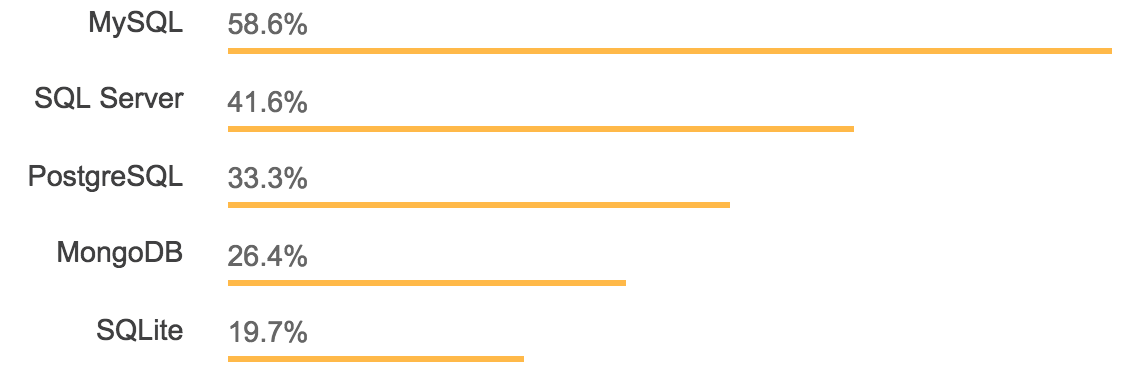
\includegraphics[width=.85\linewidth]{stackoverflow}
	\caption[Usage of the storage technologies]{Top five most commonly used storage systems, according to \textit{Stack overflow}'s Developer survey 2018\label{fig:stackoverflow}}
\end{figure}


A powerful way to overcome this representational limitations is to use \textit{predicate logic} as a data representation format.
The field of AI combining machine learning with logic is known as \textit{Statistical relational learning} (\gls{srl}) \cite{GetoorSRL,Raedt:2016:SRA:3027718} and Inductive logic programming \cite{LucRLbook}.
These methods combine three pillars of Artificial intelligence: it uses \textit{predicate logic} to represent complex data formats, \textit{probability theory} to capture the uncertainty of reasoning and \textit{machine learning} for learning models that leverage both logic and probability from data.
This renders \gls{srl} methods amongst the most expressive AI methods, i.e., they can easily represent tabular data, networks and graphs as well as entire computer programs.



\gls{srl} formalisms have given us powerful tools to represent complex models and use them for drawing conclusion.
However, learning models from scratch has proven to be a difficult task, mostly because it includes expensive inference as a sub-procedure.
A lot of progress on learning the rules of the such logical models have been made within the \gls{ilp} community, which ignores the probabilistic aspect and focuses purely on logical aspect.
The key reason why learning is difficult for \gls{srl} models is that the learning task can be described as searching for the best predictive formulas.
However, the space of all possible formulas is huge and suffers from \textit{combinatorial explosion}.










\section{Motivations and Problem statement}

It is well known is psychology that the the ability of solving the task substantially depends on the way the task is represented.


\begin{figure}
	\centering
	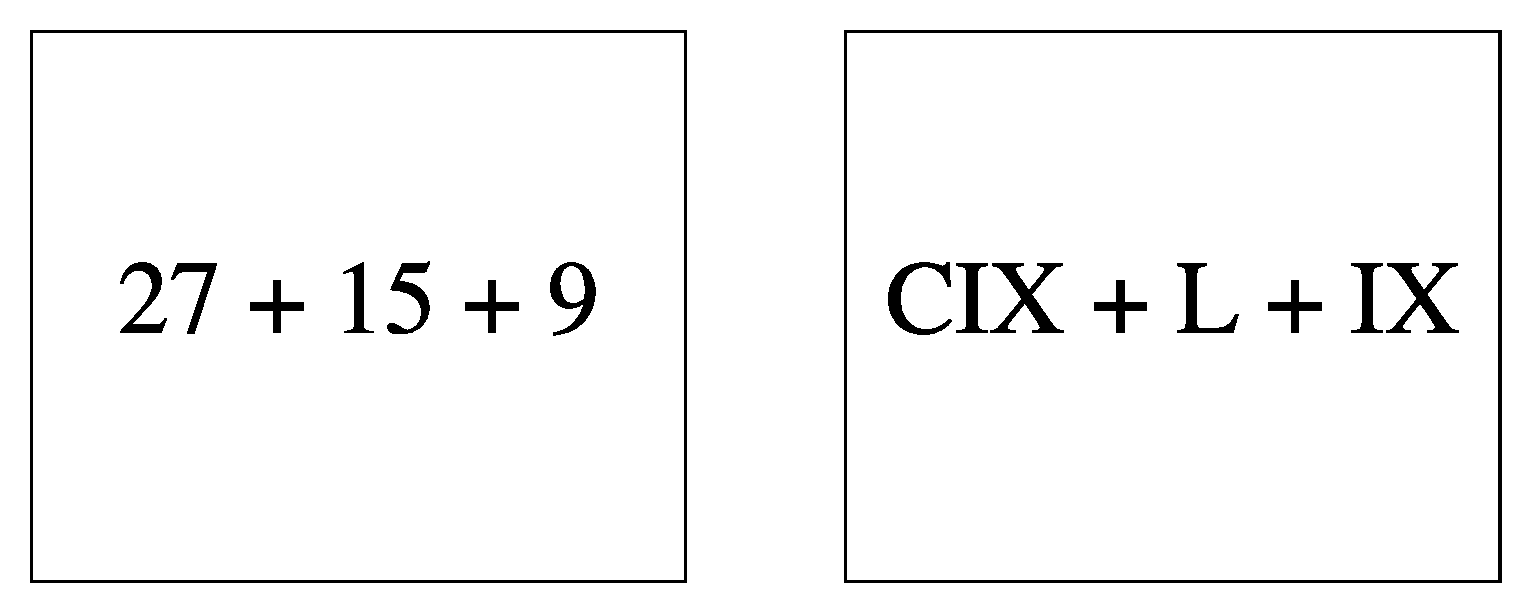
\includegraphics[width=\textwidth]{cognitiveEase}
	\caption[Cognitive ease]{\textbf{Cognitive ease.} Two tasks illustrate the concept of cognitive ease. The task on the left specifies the problem in the representation familiar to us; the task on the right a representation we can understand but are not used to. Even though both tasks are simple, the right one on average requires more effort in order to be solved.}
	\label{fig:cogease}
\end{figure}

\paragraph{Example} Consider the tasks in the Figure \ref{fig:cogease}.
These are two simple addition tasks: one with Arabic and the second one with roman numbers.
Both task are surely easy to solve.
However, paying attention to the effort it takes to solve each of the tasks, you will notice that solving the task on the right requires more effort.
Moreover, it will take you more time solve it than the task on left.
Psychologists call this \textit{cognitive ease}~\cite{kahneman2011thinking}; a measure of how easy it is for out brains to process information.
The state of cognitive ease is activated by confrontation with familiar concepts which do not require a significant effort.
The Arabic system is the system we are confronted by every day and it, thus, does not require any extensive processing effort.
In contrast, the roman system is the one we are rarely confronted with after the primary school education and thus requires a switch -- we are likely to solve it by \textit{mapping} the numbers to the Arabic system.
This task is an example of \textit{cognitive strain}.









\paragraph{Example} Consider now a typical programming task from the first-year programming course: \textit{given a collection of elements, implement a function that checks whether a given element is present in the collection}.
If the collection of elements is small, the choice of the data structure representing the collection does not matter much.
However, if the collection of elements is large, for example containing tens of millions of elements, whether a set or an array is used as a data structure makes a big difference.
Using the set representation one can check the existence of the elements almost instantly; in contrast, searching through an array results in traversing the entire collection until we find the required element.



\paragraph{Example}
Many of the objects we interact with on a daily basis are not the \textit{physical manifestation} but \textit{abstraction} that make communication easier.
For instance, a \textit{penguin} is an abstract concept, a language construct, referring to a medium-sized bird that does not fly but swims, has a beak, is of black and white colour and lives in places at the southern hemisphere.
Moreover, one can say that a bird is the abstraction of a specific group of animals that fly.
Such \textit{representation changes}, abstractions, help us to communicate effectively.
Without them, communication about categories as specific as penguin would be tedious as it would  require providing the entire definition of a category, not just a single word.




All of the examples above point to the same conclusion -- \textit{representation matters} and \textit{change of representation} is an important tool of intelligence.
The first example illustrates how even the simplest task can be made more difficult by using different representation.
The second example illustrates how change of representation can make a correct but slow solution much efficient.
Finally, the third example illustrates how introduction of abstract concepts makes communication more effective.
Unfortunately, machine learning algorithms were not capable of changing the representation autonomously until very recently.
Even the recent progress is quite limited in its scope.
Therefore, incorporating general methods for representation change into machine learning algorithms has a big potential to substantially increase their problem solving abilities.






\newglossaryentry{ann}{name={ANN},description={Artificial neural network}}
The critical limitations of the existing representation learning methods we address in this thesis are the  following.
First, the vast majority of representation learning approaches are based on the formalism of Artificial neural networks (\gls{ann}).
\gls{ann}s are known to be universal approximators, meaning that they can approximate any desired function given enough data, but are focused on tabular and signal-like data, including images, sound and text.
They are, thus, not the most suited method for relational data formats.
Consequently, the majority of representation learning approaches for relational data focuses on re-representing the data in the tabular format, which necessarily introduced a loss of information.
Second, \gls{ann}s are by their design uninterpretable.
Therefore, even though latent representation created by \gls{ann}s often perform quite well, it is often impossible to extract knowledge from the novel representation.
This undermines the trust in \gls{ml} models, especially in the domains in which interpretability is not an option but a mandatory requirement.
Third, learning representations with \gls{ann}s is often \textit{magic} --  these methods often have a large number of parameters, and their performance heavily depends on them.
Unfortunately, most of the time there is no clear guidance how to chose these parameters.







To overcome the issues outlined above, we approach the problem of learning representations of relational data from a different perspective: instead of approximating the more expressive logic framework with less expressive tabular format, we will lift the ideas from representation learning with the tabular data to the logical framework.
This view offers several benefits.
First, it  increases the \textit{expressiveness} -- what can a model represent?,  as it uses a programming language as the representation language.
Using a programming language as a representation language allows us to tackle many complicated problems which cannot be expressed in single-table format.
Moreover, programming concepts such as recursion allow us to express complicated properties in a compact manner.
Second, it is declarative.
In contrast to imperative programming paradigms which specify each step towards the solution, declarative programming paradigms specify the solution and leave it to a solver to find the correct steps.
Consequently, programs written in declarative programming languages are typically much shorter than the ones written in the imperative paradigms.
Third, it is interpretable.
Logical formulas are relatively easy to interpret for humans; that is also true for very large logical systems, if they are written in a \textit{modular} way.
This is not true for representation learning approaches based on \gls{ann}s, in which representation mapping is achieved through multiplication and addition of often millions of parameters.



Our long term goal is to develop the tools that allow \gls{ml} methods, in particular the ones within the \gls{srl} and \gls{ilp} literature, to change the representation on demand.
This will significantly reduce the effort needed from a human expert in order to find informative features for the task.
Moreover, as the goal of \gls{ai} is to develop autonomous \textit{intelligent agents} \cite{Russell:2009:AIM:1671238} capable of acting independently in the world, the ability to change the representation for the given task is an important part of it.
To contribute to the goal, this thesis explores different ideas approaching the following research question:

\begin{quote}
	How can we lift the existing representation learning techniques to the rich knowledge representation framework of predicate logic?
\end{quote}


Moreover, we will consider representation learning to be a \textit{standalone} procedure.
This view of representation learning takes data as an input of the procedure and transform the provided data to a new form, without considering the subsequent learning task.
The benefit of this view is that the latent representation of data is obtained only once and is later re-used among many tasks over the same data.







\section{Thesis contributions}




We identify \textit{four main contributions} within this thesis addressing the proposed research question.



\subsubsection{A versatile relational clustering framework}

The first main contribution of the thesis is a new \textit{versatile relational clustering method}~\cite{Dumancic2017a}.
The proposed clustering framework consists of a novel similarity measure for both objects and relationships in relational data.
The main novelty of the proposed framework is that it comprises several \textit{interpretations of similarity} of relational data, e.g. similarity in terms of attributes or structures of the neighbourhood, in contrast to the existing methods in the literature which typically impose a very strict bias on what the similarity means.
The introduced framework specified only the similarity measure and, therefore, can be further combined with any clustering algorithm.




\subsubsection{Learning latent features by detecting approximate symmetries}

The second main contribution of the thesis is a framework for learning relational latent feature by detecting \textit{approximate symmetries} in data, termed CUR$^2$LED~\cite{Dumancic2017}.
This approach is rooted in the idea that identifying similar objects in data, and finding what makes them similar, is a useful proxy towards identifying good features.
To identify the symmetries in objects and their relationships, this approach relies on the previously proposed relational clustering methods.
As knowing which kind of symmetries would be useful for a task is very difficult, if not impossible, the proposed approach makes use of many kinds of symmetries exploiting the previously introduced notion of interpretation of similarity.







\subsubsection{Auto-encoding logic programs}

The third main contribution of the thesis are \textit{auto-encoding logic programs} \cite{Dumancic2018a,AlpsSubmitted} -- a logical generalisation of auto-encoders.
Auto-encoders are among the most versatile representation learning components applicable to many different learning settings.
This versatility makes them very suitable to the variety of SRL learning tasks, such as generative modelling and supervised learning, as the same latent representation can be re-use in many tasks.
We introduce a declarative framework for learning relational auto-encoders which are implemented as logic programs, instead of matrix computation as with more standard auto-encoders.






\subsubsection{Analysis of relational representation learning approaches}

The fourth contribution of this thesis is the empirical analysis and comparison of several relational representation learning methods.
First, we focus on better understanding CUR$^2$LED and show that the created latent features match well with the existing labels, which explains why such latent features are beneficial.
Second, we compare symbolic relational learning approaches to the prototypical \textit{knowledge graph embedding methods} -- a novel paradigm for relational learning rooted in representation learning, which approaches the problem by mapping logical symbols to points in Euclidean space.
We compare their performance on various relational datasets, identify their strengths and weaknesses and show that a good idea might be to have a hybrid learner exploit the strengths of both sides.








\section{Structure of the thesis}


The work in this theses combines the fields of \textit{statistical relational learning} and \textit{representation learning}.
We review the basic foundations of Statistical Relational learning in \textbf{Chapter \ref{ch:learninglogic}} and Representation learning in \textbf{Chapter \ref{ch:learningrepresentations}}.


\textbf{Chapter \ref{ch:clustering}} presents a versatile clustering framework for relational data.
The key contributions of this chapter are (i) a novel similarity measure for relational objects, based on the summarisation of neighbourhood of individual objects, and (ii) a general framework for clustering both objects and relationships in the data.
The major novelty of the proposed framework is that it relies on several ways to define a similarity, instead of using only one way to look at it.
This chapter is based on the following publication

\begin{quote}
	\bibentry{Dumancic2017a}
\end{quote}





The following chapters explore different ideas towards learning relational latent features.
\textbf{Chapter \ref{ch:symmetries}} introduces the idea of using approximate symmetries in data as a latent representation of data.
It relies on the previously introduced relational clustering framework to identify various approximate symmetries, i.e. groups of relational objects that are \textit{similar} but not \textit{identical} to each other, and treats the identified symmetries as latent features.
Furthermore, it introduces a method for explaining the created latent features.
\textbf{Chapter \ref{ch:alps}} introduces \textit{auto-encoding logic programs}, a declarative generalisation of the auto-encoder architecture \cite{Hinton504} that uses logic programs as a computational framework.
It introduces a general modelling framework for auto-encoding logic programs, as well as a general solver based on the constraint satisfaction problem that learns them from the declarative models provided by the user.
These chapters are based on the following publications:

\begin{quote}
	\bibentry{Dumancic2017}
\end{quote}

\begin{quote}
	\bibentry{Dumancic2017b}
\end{quote}

\begin{quote}
	\bibentry{Dumancic2018a}
\end{quote}

\begin{quote}
	\bibentry{AlpsSubmitted}
\end{quote}


\textbf{Chapter \ref{ch:embeddinganalysis}} summarises the insights found by comparing various relational representation learning methods.
The analysis focuses on identifying strengths and weaknesses of various methods, as well as conditions under which different methods are applicable.
This chapter is based on the following publications

\begin{quote}
	\bibentry{Dumancic2017b}
\end{quote}

\begin{quote}
	\bibentry{Dumancic2018}
\end{quote}

\begin{quote}
	\bibentry{AnalysisSubmitted}
\end{quote}


The final chapter summarises the thesis, discusses its implications and provides a look into directions for \textit{future work}.







%%%%%%%%%%%%%%%%%%%%%%%%%%%%%%%%%%%%%%%%%%%%%%%%%%
% Keep the following \cleardoublepage at the end of this file,
% otherwise \includeonly includes empty pages.
\cleardoublepage

% vim: tw=70 nocindent expandtab foldmethod=marker foldmarker={{{}{,}{}}}
